\chapter{木に対するクエリ - Tree queries}

\index{木に対するクエリ - tree query}

ここでは根付き木における部分木とパスに関するクエリについて説明します。
例えば次のようなクエリを取り上げます。

\begin{itemize}
\item $k$番目の祖先(ancestor)はどのノード?
\item ある部分木の値の合計は?
\item 2つのノード間のパス上の値の和は?
\item 2つのノードの共通祖先(LCA)は?
\end{itemize}

\section{祖先の検索 - Finding ancestors}

\index{祖先 - ancestor}

根付き木においてノード$x$の$k$番目の祖先とは
$x$から$k$個だけ根の方向に移動したときのノードです。
ノード$x$の$k$番目の祖先を$ancestor(x, k)$とします。(祖先が存在しない場合は0とする)。
たとえば、次の木では、
$\texttt{ancestor}(2,1)=1$ and $\texttt{ancestor}(8,2)=4$です。

\begin{center}
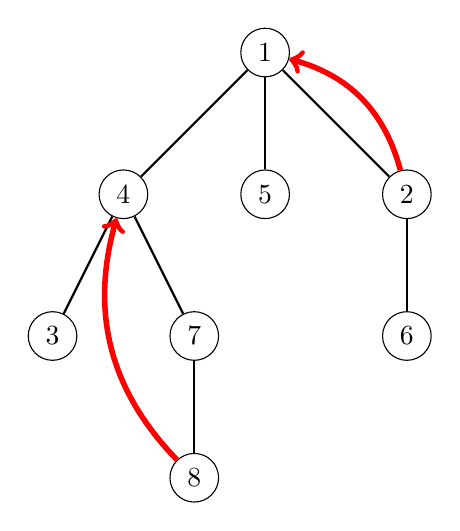
\begin{tikzpicture}[scale=0.9]
\node[draw, circle] (1) at (0,3) {$1$};
\node[draw, circle] (2) at (2,1) {$2$};
\node[draw, circle] (3) at (-2,1) {$4$};
\node[draw, circle] (4) at (0,1) {$5$};
\node[draw, circle] (5) at (2,-1) {$6$};
\node[draw, circle] (6) at (-3,-1) {$3$};
\node[draw, circle] (7) at (-1,-1) {$7$};
\node[draw, circle] (8) at (-1,-3) {$8$};
\path[draw,thick,-] (1) -- (2);
\path[draw,thick,-] (1) -- (3);
\path[draw,thick,-] (1) -- (4);
\path[draw,thick,-] (2) -- (5);
\path[draw,thick,-] (3) -- (6);
\path[draw,thick,-] (3) -- (7);
\path[draw,thick,-] (7) -- (8);

\path[draw=red,thick,->,line width=2pt] (8) edge [bend left] (3);
\path[draw=red,thick,->,line width=2pt] (2) edge [bend right] (1);
\end{tikzpicture}
\end{center}

$ancestor$を求める最もシンプルな方法は$k$回の移動を実際に行うことです。
この方法の時間計算量は$O(k)$であり、$n$ 個のノード を持つ木では$n$個のノードの探索を持つ可能性があるため、高速に動作するとは言えません。

ここで16.3章で用いたのと同様の手法を用いれば、前処理を行うことで$ancestor(x, k)$を$O(\log k)$で効率的に求められます。
$k \le n$となる$2$の累乗について$ancestor(x, k)$を事前計算します。例えば、上記の木に対する値は以下の通りになります。

\begin{center}
\begin{tabular}{r|rrrrrrrrr}
$x$ & 1 & 2 & 3 & 4 & 5 & 6 & 7 & 8 \\
\hline
$\texttt{ancestor}(x,1)$ & 0 & 1 & 4 & 1 & 1 & 2 & 4 & 7 \\
$\texttt{ancestor}(x,2)$ & 0 & 0 & 1 & 0 & 0 & 1 & 1 & 4 \\
$\texttt{ancestor}(x,4)$ & 0 & 0 & 0 & 0 & 0 & 0 & 0 & 0 \\
$\cdots$ \\
\end{tabular}
\end{center}

この前処理には各ノードに対して$O(\log n)$の計算が必要なので$O(n \log n)$の時間がかかります。
この後、$ancestor(x, k)$ の任意の値は、$k$ を各項が2のべき乗である和として表現することで$O(\log k)$で計算可能となります。

\section{部分木とパス - Subtrees and paths}

\index{tree traversal array}

\key{木の探索順 - tree traversal array}は根をもつ木のノードを、
ルートノードからの深さ優先探索 で訪れる順番に並べたものです。

\begin{center}
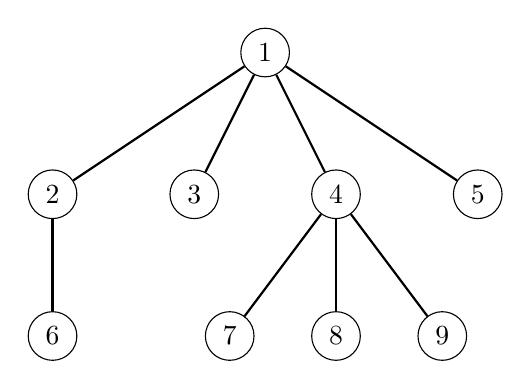
\begin{tikzpicture}[scale=0.9]
\node[draw, circle] (1) at (0,3) {$1$};
\node[draw, circle] (2) at (-3,1) {$2$};
\node[draw, circle] (3) at (-1,1) {$3$};
\node[draw, circle] (4) at (1,1) {$4$};
\node[draw, circle] (5) at (3,1) {$5$};
\node[draw, circle] (6) at (-3,-1) {$6$};
\node[draw, circle] (7) at (-0.5,-1) {$7$};
\node[draw, circle] (8) at (1,-1) {$8$};
\node[draw, circle] (9) at (2.5,-1) {$9$};

\path[draw,thick,-] (1) -- (2);
\path[draw,thick,-] (1) -- (3);
\path[draw,thick,-] (1) -- (4);
\path[draw,thick,-] (1) -- (5);
\path[draw,thick,-] (2) -- (6);
\path[draw,thick,-] (4) -- (7);
\path[draw,thick,-] (4) -- (8);
\path[draw,thick,-] (4) -- (9);
\end{tikzpicture}
\end{center}
このような場合は深さ優先探索を行い、
\begin{center}
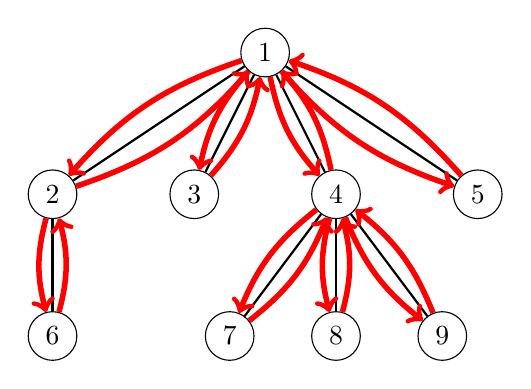
\begin{tikzpicture}[scale=0.9]
\node[draw, circle] (1) at (0,3) {$1$};
\node[draw, circle] (2) at (-3,1) {$2$};
\node[draw, circle] (3) at (-1,1) {$3$};
\node[draw, circle] (4) at (1,1) {$4$};
\node[draw, circle] (5) at (3,1) {$5$};
\node[draw, circle] (6) at (-3,-1) {$6$};
\node[draw, circle] (7) at (-0.5,-1) {$7$};
\node[draw, circle] (8) at (1,-1) {$8$};
\node[draw, circle] (9) at (2.5,-1) {$9$};

\path[draw,thick,-] (1) -- (2);
\path[draw,thick,-] (1) -- (3);
\path[draw,thick,-] (1) -- (4);
\path[draw,thick,-] (1) -- (5);
\path[draw,thick,-] (2) -- (6);
\path[draw,thick,-] (4) -- (7);
\path[draw,thick,-] (4) -- (8);
\path[draw,thick,-] (4) -- (9);


\path[draw=red,thick,->,line width=2pt] (1) edge [bend right=15] (2);
\path[draw=red,thick,->,line width=2pt] (2) edge [bend right=15] (6);
\path[draw=red,thick,->,line width=2pt] (6) edge [bend right=15] (2);
\path[draw=red,thick,->,line width=2pt] (2) edge [bend right=15] (1);
\path[draw=red,thick,->,line width=2pt] (1) edge [bend right=15] (3);
\path[draw=red,thick,->,line width=2pt] (3) edge [bend right=15] (1);
\path[draw=red,thick,->,line width=2pt] (1) edge [bend right=15] (4);
\path[draw=red,thick,->,line width=2pt] (4) edge [bend right=15] (7);
\path[draw=red,thick,->,line width=2pt] (7) edge [bend right=15] (4);
\path[draw=red,thick,->,line width=2pt] (4) edge [bend right=15] (8);
\path[draw=red,thick,->,line width=2pt] (8) edge [bend right=15] (4);
\path[draw=red,thick,->,line width=2pt] (4) edge [bend right=15] (9);
\path[draw=red,thick,->,line width=2pt] (9) edge [bend right=15] (4);
\path[draw=red,thick,->,line width=2pt] (4) edge [bend right=15] (1);
\path[draw=red,thick,->,line width=2pt] (1) edge [bend right=15] (5);
\path[draw=red,thick,->,line width=2pt] (5) edge [bend right=15] (1);

\end{tikzpicture}
\end{center}
このように辿るため、木の探索順は次のようになります。
\begin{center}
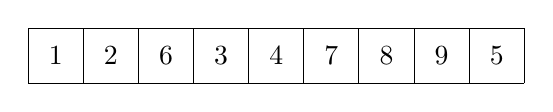
\begin{tikzpicture}[scale=0.7]
\draw (0,0) grid (9,1);

\node at (0.5,0.5) {$1$};
\node at (1.5,0.5) {$2$};
\node at (2.5,0.5) {$6$};
\node at (3.5,0.5) {$3$};
\node at (4.5,0.5) {$4$};
\node at (5.5,0.5) {$7$};
\node at (6.5,0.5) {$8$};
\node at (7.5,0.5) {$9$};
\node at (8.5,0.5) {$5$};
%
% \footnotesize
% \node at (0.5,1.4) {$1$};
% \node at (1.5,1.4) {$2$};
% \node at (2.5,1.4) {$3$};
% \node at (3.5,1.4) {$4$};
% \node at (4.5,1.4) {$5$};
% \node at (5.5,1.4) {$6$};
% \node at (6.5,1.4) {$7$};
% \node at (7.5,1.4) {$8$};
% \node at (8.5,1.4) {$9$};
\end{tikzpicture}
\end{center}

\subsubsection{部分木クエリ - Subtree queries}

木における部分木は、木の探索順のある部分配列に対応し、
その部分配列の 最初の要素がその部分木の根となるようにします。
例えば、以下の部分配列は、ノード $4$ の部分木となります。

\begin{center}
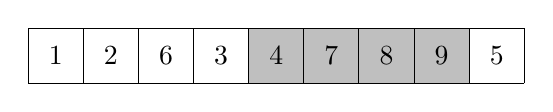
\begin{tikzpicture}[scale=0.7]
\fill[color=lightgray] (4,0) rectangle (8,1);
\draw (0,0) grid (9,1);

\node at (0.5,0.5) {$1$};
\node at (1.5,0.5) {$2$};
\node at (2.5,0.5) {$6$};
\node at (3.5,0.5) {$3$};
\node at (4.5,0.5) {$4$};
\node at (5.5,0.5) {$7$};
\node at (6.5,0.5) {$8$};
\node at (7.5,0.5) {$9$};
\node at (8.5,0.5) {$5$};
%
% \footnotesize
% \node at (0.5,1.4) {$1$};
% \node at (1.5,1.4) {$2$};
% \node at (2.5,1.4) {$3$};
% \node at (3.5,1.4) {$4$};
% \node at (4.5,1.4) {$5$};
% \node at (5.5,1.4) {$6$};
% \node at (6.5,1.4) {$7$};
% \node at (7.5,1.4) {$8$};
% \node at (8.5,1.4) {$9$};
\end{tikzpicture}
\end{center}

これを利用して、木の部分木対するクエリを効率的に処理できます。
例として、各ノードに値があるとします。次のようなクエリを考えます。
\begin{itemize}
\item 単一ノードの値を更新する
\item 単一の指定したノードの部分木の合計を計算する
\end{itemize}

次の図で青い数字がノードの値とします。例えば、ノード $4$の部分木の和は、$3+ 4+ 3+ 1= 11$となります。

\begin{center}
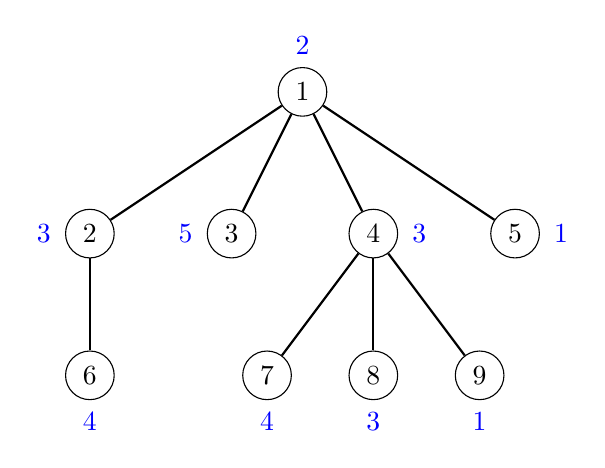
\begin{tikzpicture}[scale=0.9]
\node[draw, circle] (1) at (0,3) {$1$};
\node[draw, circle] (2) at (-3,1) {$2$};
\node[draw, circle] (3) at (-1,1) {$3$};
\node[draw, circle] (4) at (1,1) {$4$};
\node[draw, circle] (5) at (3,1) {$5$};
\node[draw, circle] (6) at (-3,-1) {$6$};
\node[draw, circle] (7) at (-0.5,-1) {$7$};
\node[draw, circle] (8) at (1,-1) {$8$};
\node[draw, circle] (9) at (2.5,-1) {$9$};

\path[draw,thick,-] (1) -- (2);
\path[draw,thick,-] (1) -- (3);
\path[draw,thick,-] (1) -- (4);
\path[draw,thick,-] (1) -- (5);
\path[draw,thick,-] (2) -- (6);
\path[draw,thick,-] (4) -- (7);
\path[draw,thick,-] (4) -- (8);
\path[draw,thick,-] (4) -- (9);

\node[color=blue] at (0,3+0.65) {2};
\node[color=blue] at (-3-0.65,1) {3};
\node[color=blue] at (-1-0.65,1) {5};
\node[color=blue] at (1+0.65,1) {3};
\node[color=blue] at (3+0.65,1) {1};
\node[color=blue] at (-3,-1-0.65) {4};
\node[color=blue] at (-0.5,-1-0.65) {4};
\node[color=blue] at (1,-1-0.65) {3};
\node[color=blue] at (2.5,-1-0.65) {1};
\end{tikzpicture}
\end{center}

この問題を解くアイデアは各ノードに対して、ノードの番号、サブツリーのサイズ、ノードの値を持っておきます。
次のようになります。

\begin{center}
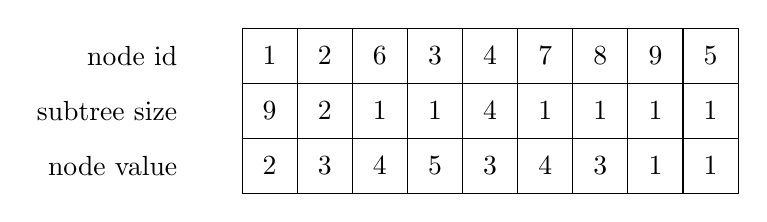
\begin{tikzpicture}[scale=0.7]
\draw (0,1) grid (9,-2);

\node[left] at (-1,0.5) {node id};
\node[left] at (-1,-0.5) {subtree size};
\node[left] at (-1,-1.5) {node value};

\node at (0.5,0.5) {$1$};
\node at (1.5,0.5) {$2$};
\node at (2.5,0.5) {$6$};
\node at (3.5,0.5) {$3$};
\node at (4.5,0.5) {$4$};
\node at (5.5,0.5) {$7$};
\node at (6.5,0.5) {$8$};
\node at (7.5,0.5) {$9$};
\node at (8.5,0.5) {$5$};

\node at (0.5,-0.5) {$9$};
\node at (1.5,-0.5) {$2$};
\node at (2.5,-0.5) {$1$};
\node at (3.5,-0.5) {$1$};
\node at (4.5,-0.5) {$4$};
\node at (5.5,-0.5) {$1$};
\node at (6.5,-0.5) {$1$};
\node at (7.5,-0.5) {$1$};
\node at (8.5,-0.5) {$1$};

\node at (0.5,-1.5) {$2$};
\node at (1.5,-1.5) {$3$};
\node at (2.5,-1.5) {$4$};
\node at (3.5,-1.5) {$5$};
\node at (4.5,-1.5) {$3$};
\node at (5.5,-1.5) {$4$};
\node at (6.5,-1.5) {$3$};
\node at (7.5,-1.5) {$1$};
\node at (8.5,-1.5) {$1$};
%
% \footnotesize
% \node at (0.5,1.4) {$1$};
% \node at (1.5,1.4) {$2$};
% \node at (2.5,1.4) {$3$};
% \node at (3.5,1.4) {$4$};
% \node at (4.5,1.4) {$5$};
% \node at (5.5,1.4) {$6$};
% \node at (6.5,1.4) {$7$};
% \node at (7.5,1.4) {$8$};
% \node at (8.5,1.4) {$9$};
\end{tikzpicture}
\end{center}


この配列によって、まずサブツリーの大きさを求め、
次に対応するノードの値を求めれば、任意の部分木の値の合計を計算することができます。
ノード$4$の部分木の値は以下のように求めます。

\begin{center}
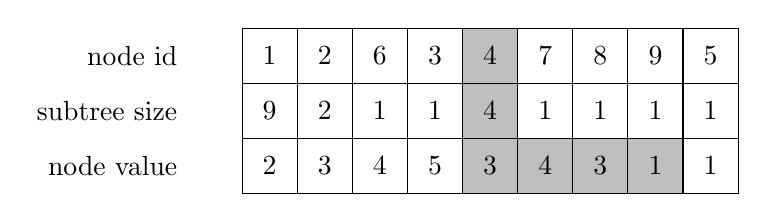
\begin{tikzpicture}[scale=0.7]
\fill[color=lightgray] (4,1) rectangle (5,0);
\fill[color=lightgray] (4,0) rectangle (5,-1);
\fill[color=lightgray] (4,-1) rectangle (8,-2);
\draw (0,1) grid (9,-2);

\node[left] at (-1,0.5) {node id};
\node[left] at (-1,-0.5) {subtree size};
\node[left] at (-1,-1.5) {node value};

\node at (0.5,0.5) {$1$};
\node at (1.5,0.5) {$2$};
\node at (2.5,0.5) {$6$};
\node at (3.5,0.5) {$3$};
\node at (4.5,0.5) {$4$};
\node at (5.5,0.5) {$7$};
\node at (6.5,0.5) {$8$};
\node at (7.5,0.5) {$9$};
\node at (8.5,0.5) {$5$};

\node at (0.5,-0.5) {$9$};
\node at (1.5,-0.5) {$2$};
\node at (2.5,-0.5) {$1$};
\node at (3.5,-0.5) {$1$};
\node at (4.5,-0.5) {$4$};
\node at (5.5,-0.5) {$1$};
\node at (6.5,-0.5) {$1$};
\node at (7.5,-0.5) {$1$};
\node at (8.5,-0.5) {$1$};

\node at (0.5,-1.5) {$2$};
\node at (1.5,-1.5) {$3$};
\node at (2.5,-1.5) {$4$};
\node at (3.5,-1.5) {$5$};
\node at (4.5,-1.5) {$3$};
\node at (5.5,-1.5) {$4$};
\node at (6.5,-1.5) {$3$};
\node at (7.5,-1.5) {$1$};
\node at (8.5,-1.5) {$1$};
%
% \footnotesize
% \node at (0.5,1.4) {$1$};
% \node at (1.5,1.4) {$2$};
% \node at (2.5,1.4) {$3$};
% \node at (3.5,1.4) {$4$};
% \node at (4.5,1.4) {$5$};
% \node at (5.5,1.4) {$6$};
% \node at (6.5,1.4) {$7$};
% \node at (7.5,1.4) {$8$};
% \node at (8.5,1.4) {$9$};
\end{tikzpicture}
\end{center}

クエリに効率的に答えるにはこれを格納する構造体を工夫することが必要です。
バイナリインデックスまたはセグメントツリーなどが適切でしょう。
これらを用いると値の更新と値の総和の計算の両方を$O(\log n)$で行うことができます。


\subsubsection{パスクエリ - Path queries}


また、木の探索順を用いると、根から木の任意のノードまでのパスの値の総和を効率的に計算することができます。
次のようなクエリを考えましょう。

\begin{itemize}
\item 単一ノードの値を変更する
\item 根から単一ノードへの値の総和を考える
\end{itemize}

例えば、次の図では根からノード$7$へのコストは$4+5+5=14$となります。

\begin{center}
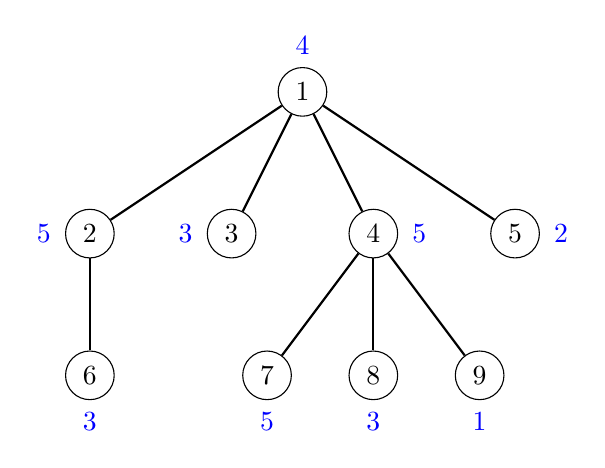
\begin{tikzpicture}[scale=0.9]
\node[draw, circle] (1) at (0,3) {$1$};
\node[draw, circle] (2) at (-3,1) {$2$};
\node[draw, circle] (3) at (-1,1) {$3$};
\node[draw, circle] (4) at (1,1) {$4$};
\node[draw, circle] (5) at (3,1) {$5$};
\node[draw, circle] (6) at (-3,-1) {$6$};
\node[draw, circle] (7) at (-0.5,-1) {$7$};
\node[draw, circle] (8) at (1,-1) {$8$};
\node[draw, circle] (9) at (2.5,-1) {$9$};

\path[draw,thick,-] (1) -- (2);
\path[draw,thick,-] (1) -- (3);
\path[draw,thick,-] (1) -- (4);
\path[draw,thick,-] (1) -- (5);
\path[draw,thick,-] (2) -- (6);
\path[draw,thick,-] (4) -- (7);
\path[draw,thick,-] (4) -- (8);
\path[draw,thick,-] (4) -- (9);

\node[color=blue] at (0,3+0.65) {4};
\node[color=blue] at (-3-0.65,1) {5};
\node[color=blue] at (-1-0.65,1) {3};
\node[color=blue] at (1+0.65,1) {5};
\node[color=blue] at (3+0.65,1) {2};
\node[color=blue] at (-3,-1-0.65) {3};
\node[color=blue] at (-0.5,-1-0.65) {5};
\node[color=blue] at (1,-1-0.65) {3};
\node[color=blue] at (2.5,-1-0.65) {1};
\end{tikzpicture}
\end{center}

これは先ほど同様に解くことができますが、
今度は配列の最後の行の各値が、ルートからノードへのパス上の値の合計となります。

We can solve this problem like before,
but now each value in the last row of the array is the sum of values
on a path from the root to the node.
For example, the following array corresponds to the above tree:
\begin{center}
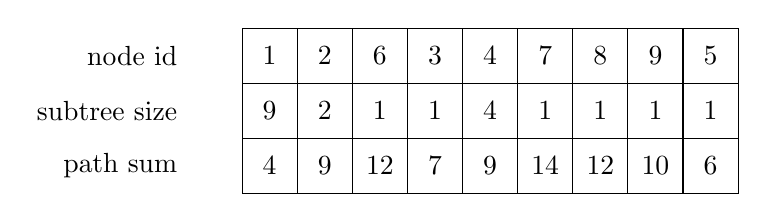
\begin{tikzpicture}[scale=0.7]
\draw (0,1) grid (9,-2);

\node[left] at (-1,0.5) {node id};
\node[left] at (-1,-0.5) {subtree size};
\node[left] at (-1,-1.5) {path sum};

\node at (0.5,0.5) {$1$};
\node at (1.5,0.5) {$2$};
\node at (2.5,0.5) {$6$};
\node at (3.5,0.5) {$3$};
\node at (4.5,0.5) {$4$};
\node at (5.5,0.5) {$7$};
\node at (6.5,0.5) {$8$};
\node at (7.5,0.5) {$9$};
\node at (8.5,0.5) {$5$};

\node at (0.5,-0.5) {$9$};
\node at (1.5,-0.5) {$2$};
\node at (2.5,-0.5) {$1$};
\node at (3.5,-0.5) {$1$};
\node at (4.5,-0.5) {$4$};
\node at (5.5,-0.5) {$1$};
\node at (6.5,-0.5) {$1$};
\node at (7.5,-0.5) {$1$};
\node at (8.5,-0.5) {$1$};

\node at (0.5,-1.5) {$4$};
\node at (1.5,-1.5) {$9$};
\node at (2.5,-1.5) {$12$};
\node at (3.5,-1.5) {$7$};
\node at (4.5,-1.5) {$9$};
\node at (5.5,-1.5) {$14$};
\node at (6.5,-1.5) {$12$};
\node at (7.5,-1.5) {$10$};
\node at (8.5,-1.5) {$6$};
\end{tikzpicture}
\end{center}

あるノードの値が$x$増加した時、そのサブツリーの値は全て$x$増加します。
例えば、ノード4が1増加した時、以下のように変化が起こります。

\begin{center}
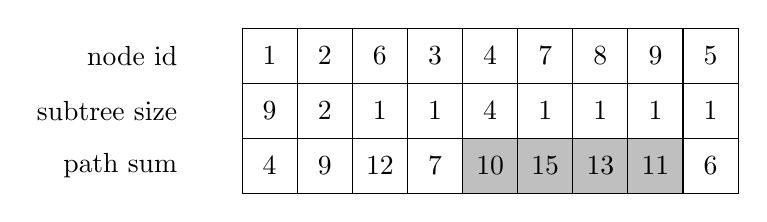
\begin{tikzpicture}[scale=0.7]
\fill[color=lightgray] (4,-1) rectangle (8,-2);
\draw (0,1) grid (9,-2);

\node[left] at (-1,0.5) {node id};
\node[left] at (-1,-0.5) {subtree size};
\node[left] at (-1,-1.5) {path sum};

\node at (0.5,0.5) {$1$};
\node at (1.5,0.5) {$2$};
\node at (2.5,0.5) {$6$};
\node at (3.5,0.5) {$3$};
\node at (4.5,0.5) {$4$};
\node at (5.5,0.5) {$7$};
\node at (6.5,0.5) {$8$};
\node at (7.5,0.5) {$9$};
\node at (8.5,0.5) {$5$};

\node at (0.5,-0.5) {$9$};
\node at (1.5,-0.5) {$2$};
\node at (2.5,-0.5) {$1$};
\node at (3.5,-0.5) {$1$};
\node at (4.5,-0.5) {$4$};
\node at (5.5,-0.5) {$1$};
\node at (6.5,-0.5) {$1$};
\node at (7.5,-0.5) {$1$};
\node at (8.5,-0.5) {$1$};

\node at (0.5,-1.5) {$4$};
\node at (1.5,-1.5) {$9$};
\node at (2.5,-1.5) {$12$};
\node at (3.5,-1.5) {$7$};
\node at (4.5,-1.5) {$10$};
\node at (5.5,-1.5) {$15$};
\node at (6.5,-1.5) {$13$};
\node at (7.5,-1.5) {$11$};
\node at (8.5,-1.5) {$6$};
\end{tikzpicture}
\end{center}

この2つの操作をサポートするためには、区間更新が可能である値が取り出すデータ構造が必要です。
これは、バイナリインデックスまたはセグメントツリーを使用して$O(\log n)$時間で行うことができます
(9.4章参照)。

\section{最小共通祖先(LCA) - Lowest common ancestor}

\index{最小共通祖先(LCA) - lowest common ancestor}

根付き木の2つのノードの\key{最小共通祖先(LCA) - lowest common ancestor}とは、
あるノードの部分木が2つのノードを含むような最も下のノードのことです。
最も典型的な問題は2つのノードのペアが与えられるのでその問い合わせを効率的に行う問題です。
例えば、以下の木では、ノード$5$と$8$のLCAはノード2です。

\begin{center}
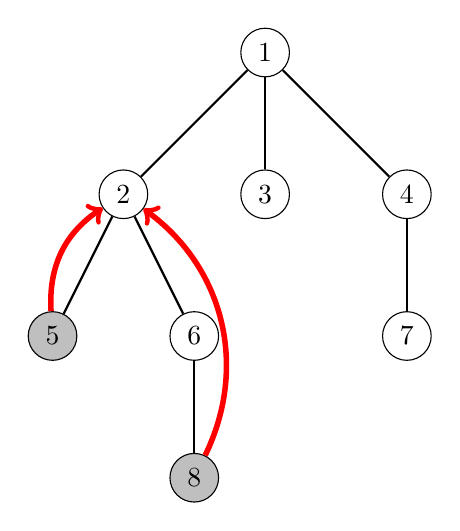
\begin{tikzpicture}[scale=0.9]
\node[draw, circle] (1) at (0,3) {$1$};
\node[draw, circle] (2) at (2,1) {$4$};
\node[draw, circle] (3) at (-2,1) {$2$};
\node[draw, circle] (4) at (0,1) {$3$};
\node[draw, circle] (5) at (2,-1) {$7$};
\node[draw, circle, fill=lightgray] (6) at (-3,-1) {$5$};
\node[draw, circle] (7) at (-1,-1) {$6$};
\node[draw, circle, fill=lightgray] (8) at (-1,-3) {$8$};
\path[draw,thick,-] (1) -- (2);
\path[draw,thick,-] (1) -- (3);
\path[draw,thick,-] (1) -- (4);
\path[draw,thick,-] (2) -- (5);
\path[draw,thick,-] (3) -- (6);
\path[draw,thick,-] (3) -- (7);
\path[draw,thick,-] (7) -- (8);

\path[draw=red,thick,->,line width=2pt] (6) edge [bend left] (3);
\path[draw=red,thick,->,line width=2pt] (8) edge [bend right=40] (3);
\end{tikzpicture}
\end{center}

さて、LCAを求めるための2つの方法を紹介します。

\subsubsection{手法1: ダブリング - Method 1}

1つめの方法では、先ほど紹介した木の任意のノードの$k$番目の先祖は効率的に見つけることができる性質を利用します。
これを利用してLCAを2つの問題として捉えられます。
2つのポインタを使い、最初は対象の2つのノードを指します。
ここで深い方のポインタの一方を上方に移動させ、両方のポインタが同じ深さとなるようにします。
以下の2番目のポインタを1レベル上げて、ノード5と同じ深さにあるノード6を指すようにします。

\begin{center}
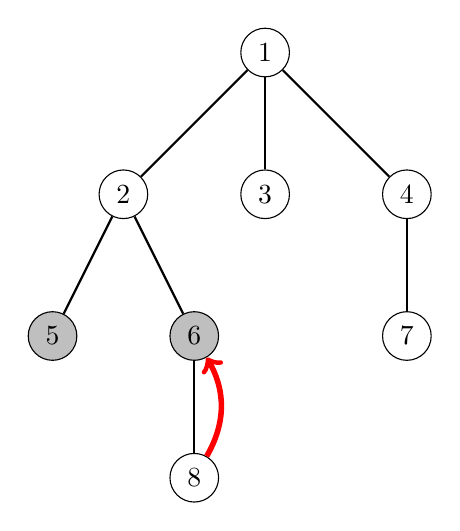
\begin{tikzpicture}[scale=0.9]
\node[draw, circle] (1) at (0,3) {$1$};
\node[draw, circle] (2) at (2,1) {$4$};
\node[draw, circle] (3) at (-2,1) {$2$};
\node[draw, circle] (4) at (0,1) {$3$};
\node[draw, circle] (5) at (2,-1) {$7$};
\node[draw, circle,fill=lightgray] (6) at (-3,-1) {$5$};
\node[draw, circle,fill=lightgray] (7) at (-1,-1) {$6$};
\node[draw, circle] (8) at (-1,-3) {$8$};
\path[draw,thick,-] (1) -- (2);
\path[draw,thick,-] (1) -- (3);
\path[draw,thick,-] (1) -- (4);
\path[draw,thick,-] (2) -- (5);
\path[draw,thick,-] (3) -- (6);
\path[draw,thick,-] (3) -- (7);
\path[draw,thick,-] (7) -- (8);

\path[draw=red,thick,->,line width=2pt] (8) edge [bend right] (7);
\end{tikzpicture}
\end{center}

次に、両者のポインタを上方に移動させ、同じノードを指すようにするために必要な最小のステップ数を求めます。
この後、ポインタが指すノードがLCAとなります。
この例では、両方のポインタを一段階上のノード2(LCA)に移動させることになります。

\begin{center}
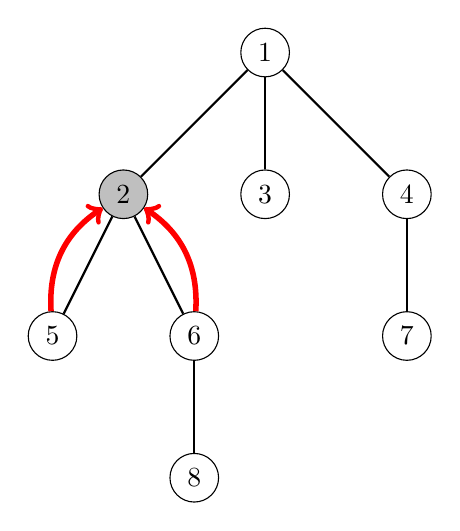
\begin{tikzpicture}[scale=0.9]
\node[draw, circle] (1) at (0,3) {$1$};
\node[draw, circle] (2) at (2,1) {$4$};
\node[draw, circle,fill=lightgray] (3) at (-2,1) {$2$};
\node[draw, circle] (4) at (0,1) {$3$};
\node[draw, circle] (5) at (2,-1) {$7$};
\node[draw, circle] (6) at (-3,-1) {$5$};
\node[draw, circle] (7) at (-1,-1) {$6$};
\node[draw, circle] (8) at (-1,-3) {$8$};
\path[draw,thick,-] (1) -- (2);
\path[draw,thick,-] (1) -- (3);
\path[draw,thick,-] (1) -- (4);
\path[draw,thick,-] (2) -- (5);
\path[draw,thick,-] (3) -- (6);
\path[draw,thick,-] (3) -- (7);
\path[draw,thick,-] (7) -- (8);

\path[draw=red,thick,->,line width=2pt] (6) edge [bend left] (3);
\path[draw=red,thick,->,line width=2pt] (7) edge [bend right] (3);
\end{tikzpicture}
\end{center}

このアルゴリズムは事前に計算された情報を使って$O(\log n)$ 時間で実行できるので、
任意の2つのノードのLCAは$O(\log n)$で見つけることができます。

\subsubsection{手法2: オイラーツアー - Method 2}


この方法は木の探索順によってLCAを求めます。\footnote{This lowest common ancestor algorithm was presented in \cite{ben00}.
This technique is sometimes called the \index{Euler tour technique}
\key{Euler tour technique} \cite{tar84}.}
これは深さ優先探索を有効に使う方法です。

\begin{center}
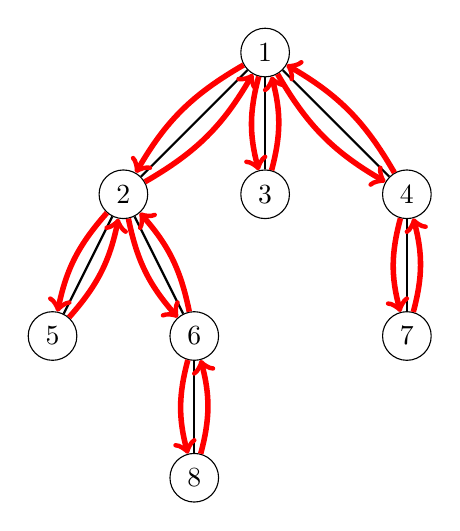
\begin{tikzpicture}[scale=0.9]
\node[draw, circle] (1) at (0,3) {$1$};
\node[draw, circle] (2) at (2,1) {$4$};
\node[draw, circle] (3) at (-2,1) {$2$};
\node[draw, circle] (4) at (0,1) {$3$};
\node[draw, circle] (5) at (2,-1) {$7$};
\node[draw, circle] (6) at (-3,-1) {$5$};
\node[draw, circle] (7) at (-1,-1) {$6$};
\node[draw, circle] (8) at (-1,-3) {$8$};
\path[draw,thick,-] (1) -- (2);
\path[draw,thick,-] (1) -- (3);
\path[draw,thick,-] (1) -- (4);
\path[draw,thick,-] (2) -- (5);
\path[draw,thick,-] (3) -- (6);
\path[draw,thick,-] (3) -- (7);
\path[draw,thick,-] (7) -- (8);

\path[draw=red,thick,->,line width=2pt] (1) edge [bend right=15] (3);
\path[draw=red,thick,->,line width=2pt] (3) edge [bend right=15] (6);
\path[draw=red,thick,->,line width=2pt] (6) edge [bend right=15] (3);
\path[draw=red,thick,->,line width=2pt] (3) edge [bend right=15] (7);
\path[draw=red,thick,->,line width=2pt] (7) edge [bend right=15] (8);
\path[draw=red,thick,->,line width=2pt] (8) edge [bend right=15] (7);
\path[draw=red,thick,->,line width=2pt] (7) edge [bend right=15] (3);
\path[draw=red,thick,->,line width=2pt] (3) edge [bend right=15] (1);
\path[draw=red,thick,->,line width=2pt] (1) edge [bend right=15] (4);
\path[draw=red,thick,->,line width=2pt] (4) edge [bend right=15] (1);
\path[draw=red,thick,->,line width=2pt] (1) edge [bend right=15] (2);
\path[draw=red,thick,->,line width=2pt] (2) edge [bend right=15] (5);
\path[draw=red,thick,->,line width=2pt] (5) edge [bend right=15] (2);
\path[draw=red,thick,->,line width=2pt] (2) edge [bend right=15] (1);
\end{tikzpicture}
\end{center}

ここでは先ほどと異なるのとは別の木の探索配列を使っていることに注意します。
深さ優先探索がノードを通過するときに
最初の訪問した時間だけでなく、常に各ノードを配列に追加します。
したがって、$k$個の子を持つノードは配列中に$k + 1$回出現し、
配列中には合計$2n - 1$個のノードが存在することになります。

配列には、ノードの識別子と、そのノードの木における深さを持ちます。

\begin{center}
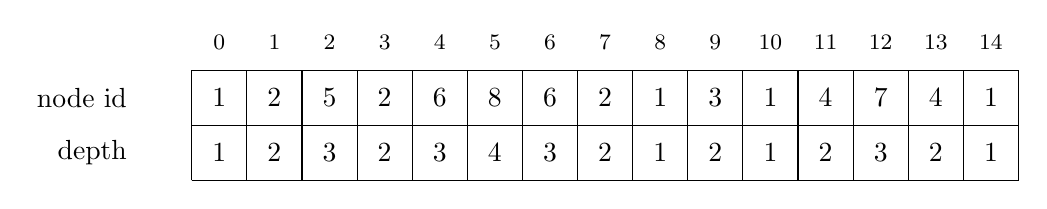
\begin{tikzpicture}[scale=0.7]

\node[left] at (-1,1.5) {node id};
\node[left] at (-1,0.5) {depth};

\draw (0,1) grid (15,2);
\node at (0.5,1.5) {$1$};
\node at (1.5,1.5) {$2$};
\node at (2.5,1.5) {$5$};
\node at (3.5,1.5) {$2$};
\node at (4.5,1.5) {$6$};
\node at (5.5,1.5) {$8$};
\node at (6.5,1.5) {$6$};
\node at (7.5,1.5) {$2$};
\node at (8.5,1.5) {$1$};
\node at (9.5,1.5) {$3$};
\node at (10.5,1.5) {$1$};
\node at (11.5,1.5) {$4$};
\node at (12.5,1.5) {$7$};
\node at (13.5,1.5) {$4$};
\node at (14.5,1.5) {$1$};

\draw (0,0) grid (15,1);
\node at (0.5,0.5) {$1$};
\node at (1.5,0.5) {$2$};
\node at (2.5,0.5) {$3$};
\node at (3.5,0.5) {$2$};
\node at (4.5,0.5) {$3$};
\node at (5.5,0.5) {$4$};
\node at (6.5,0.5) {$3$};
\node at (7.5,0.5) {$2$};
\node at (8.5,0.5) {$1$};
\node at (9.5,0.5) {$2$};
\node at (10.5,0.5) {$1$};
\node at (11.5,0.5) {$2$};
\node at (12.5,0.5) {$3$};
\node at (13.5,0.5) {$2$};
\node at (14.5,0.5) {$1$};

\footnotesize
\node at (0.5,2.5) {$0$};
\node at (1.5,2.5) {$1$};
\node at (2.5,2.5) {$2$};
\node at (3.5,2.5) {$3$};
\node at (4.5,2.5) {$4$};
\node at (5.5,2.5) {$5$};
\node at (6.5,2.5) {$6$};
\node at (7.5,2.5) {$7$};
\node at (8.5,2.5) {$8$};
\node at (9.5,2.5) {$9$};
\node at (10.5,2.5) {$10$};
\node at (11.5,2.5) {$11$};
\node at (12.5,2.5) {$12$};
\node at (13.5,2.5) {$13$};
\node at (14.5,2.5) {$14$};
\end{tikzpicture}
\end{center}

ここで、ノード$a$とノード$b$のLCAは、
配列のノード$a$とノード$b$の間の深さが最小のノードです。
例えば、ノード$5$と$8$のLCAは次のようになります。

\begin{center}
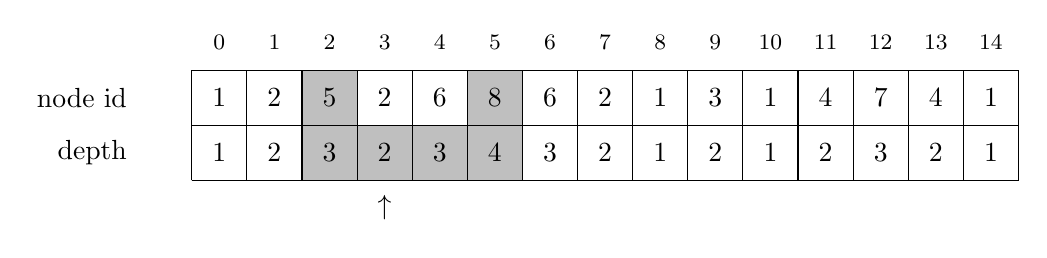
\begin{tikzpicture}[scale=0.7]

\node[left] at (-1,1.5) {node id};
\node[left] at (-1,0.5) {depth};

\fill[color=lightgray] (2,1) rectangle (3,2);
\fill[color=lightgray] (5,1) rectangle (6,2);
\fill[color=lightgray] (2,0) rectangle (6,1);

\node at (3.5,-0.5) {$\uparrow$};

\draw (0,1) grid (15,2);
\node at (0.5,1.5) {$1$};
\node at (1.5,1.5) {$2$};
\node at (2.5,1.5) {$5$};
\node at (3.5,1.5) {$2$};
\node at (4.5,1.5) {$6$};
\node at (5.5,1.5) {$8$};
\node at (6.5,1.5) {$6$};
\node at (7.5,1.5) {$2$};
\node at (8.5,1.5) {$1$};
\node at (9.5,1.5) {$3$};
\node at (10.5,1.5) {$1$};
\node at (11.5,1.5) {$4$};
\node at (12.5,1.5) {$7$};
\node at (13.5,1.5) {$4$};
\node at (14.5,1.5) {$1$};


\draw (0,0) grid (15,1);
\node at (0.5,0.5) {$1$};
\node at (1.5,0.5) {$2$};
\node at (2.5,0.5) {$3$};
\node at (3.5,0.5) {$2$};
\node at (4.5,0.5) {$3$};
\node at (5.5,0.5) {$4$};
\node at (6.5,0.5) {$3$};
\node at (7.5,0.5) {$2$};
\node at (8.5,0.5) {$1$};
\node at (9.5,0.5) {$2$};
\node at (10.5,0.5) {$1$};
\node at (11.5,0.5) {$2$};
\node at (12.5,0.5) {$3$};
\node at (13.5,0.5) {$2$};
\node at (14.5,0.5) {$1$};

\footnotesize
\node at (0.5,2.5) {$0$};
\node at (1.5,2.5) {$1$};
\node at (2.5,2.5) {$2$};
\node at (3.5,2.5) {$3$};
\node at (4.5,2.5) {$4$};
\node at (5.5,2.5) {$5$};
\node at (6.5,2.5) {$6$};
\node at (7.5,2.5) {$7$};
\node at (8.5,2.5) {$8$};
\node at (9.5,2.5) {$9$};
\node at (10.5,2.5) {$10$};
\node at (11.5,2.5) {$11$};
\node at (12.5,2.5) {$12$};
\node at (13.5,2.5) {$13$};
\node at (14.5,2.5) {$14$};
\end{tikzpicture}
\end{center}

ノード5はindex 2にあり、ノード8はindex 5にあり、
index $2 \ldots 5$の間の最小のノードを求めます
従って、ノード5とノード8のLCAは深さ2であるノード$2$となります。
2つのノードのLCAを見つけるには、区間最小を求めるクエリを処理すればよい。
配列は静的なので、$O(n \log n)$の前処理をした後、
$O(1)$時間でこのようなクエリを処理することができます。
(訳注: Sparse Tableなどを用いることでこれが実現できます)

\subsubsection{ノード間の距離 - Distances of nodes}

ノード$a$と$b$の距離とは$a$から$b$へのパスの長さです。
ノード間の距離を計算する問題は、ノード間のLCAを見つけることが大切だとわかります。
まず、木を根付きとして考えます。この後、ノード$a$、$b$の距離 は、次の式で計算できます。

\[\texttt{depth}(a)+\texttt{depth}(b)-2 \cdot \texttt{depth}(c),\]

ここで、$c$ は $a$ と $b$ のLCAノード、$\texttt{depth}(s)$ はノード $s$ の深さです。
例えば、ノード 5 と 8 の距離を考えてみます。

\begin{center}
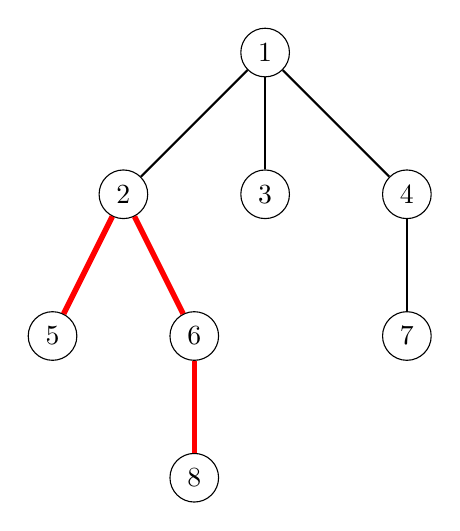
\begin{tikzpicture}[scale=0.9]
\node[draw, circle] (1) at (0,3) {$1$};
\node[draw, circle] (2) at (2,1) {$4$};
\node[draw, circle] (3) at (-2,1) {$2$};
\node[draw, circle] (4) at (0,1) {$3$};
\node[draw, circle] (5) at (2,-1) {$7$};
\node[draw, circle] (6) at (-3,-1) {$5$};
\node[draw, circle] (7) at (-1,-1) {$6$};
\node[draw, circle] (8) at (-1,-3) {$8$};
\path[draw,thick,-] (1) -- (2);
\path[draw,thick,-] (1) -- (3);
\path[draw,thick,-] (1) -- (4);
\path[draw,thick,-] (2) -- (5);
\path[draw,thick,-] (3) -- (6);
\path[draw,thick,-] (3) -- (7);
\path[draw,thick,-] (7) -- (8);

\path[draw=red,thick,-,line width=2pt] (8) -- node[font=\small] {} (7);
\path[draw=red,thick,-,line width=2pt] (7) -- node[font=\small] {} (3);
\path[draw=red,thick,-,line width=2pt] (6) -- node[font=\small] {} (3);
\end{tikzpicture}
\end{center}

ノード5と8の最小公倍数の祖先はノード2である。ノードの深さは depth(5) = 3, depth(8) = 4, depth(2) = 2 なので、 ノード 5 と 8 の間の距離は 3 + 4 - 2 - 2 = 3 である。
ノード5,8のLCAは2です。ここで、
$\texttt{depth}(5)=3$, $\texttt{depth}(8)=4$ and $\texttt{depth}(2)=2$,
であるため、5,8の距離は
$3+4-2\cdot2=3$となります。

\section{オフラインのアルゴリズム - Offline algorithms}

これまで私たちは\emph{オンライン - online}な木クエリのアルゴリズムを考えてきました。

オンラインアルゴリズムは、
次のクエリがくる前にそのクエリに応答するように、
クエリを順番に処理することができます。
これらが必要ない\emph{オフライン - offline} なアルゴリズムに注目します。
オフラインであるとは、任意の順序で回答可能な問い合わせのセットが与えられます。
つまり、最初から全てのクエリが分かっているとします。
一般にオンラインアルゴリズム と比較して、オフラインアルゴリズムの設計は容易になります。

\subsubsection{データ構造のマージ - Merging data structures}


オフラインのアルゴリズムの一例として、深さ優先の木探索によりノードにデータ構造を保持する方法があります。
各ノード$s$において、$s$の子のデー タ構造に基づくデータ構造$\texttt{d}[s]$を作成し、
このデータ構造を用いて、$s$に関連す る全ての問合せを処理していくのです。

各ノードが何らかの値を持つ木があるとします。
与えられた問題は「ノード$s$の部分木にある値$x$を持つノードの数を計算せよ」だとします。
例えば、以下の木において、ノード$4$の 部分木には値が3であるノードが2つ含まれている。

\begin{center}
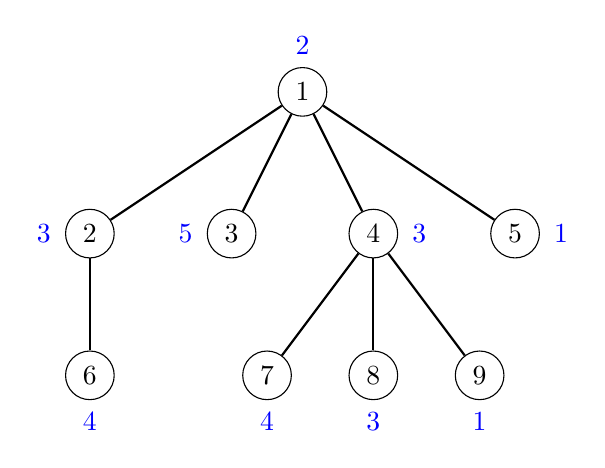
\begin{tikzpicture}[scale=0.9]
\node[draw, circle] (1) at (0,3) {$1$};
\node[draw, circle] (2) at (-3,1) {$2$};
\node[draw, circle] (3) at (-1,1) {$3$};
\node[draw, circle] (4) at (1,1) {$4$};
\node[draw, circle] (5) at (3,1) {$5$};
\node[draw, circle] (6) at (-3,-1) {$6$};
\node[draw, circle] (7) at (-0.5,-1) {$7$};
\node[draw, circle] (8) at (1,-1) {$8$};
\node[draw, circle] (9) at (2.5,-1) {$9$};

\path[draw,thick,-] (1) -- (2);
\path[draw,thick,-] (1) -- (3);
\path[draw,thick,-] (1) -- (4);
\path[draw,thick,-] (1) -- (5);
\path[draw,thick,-] (2) -- (6);
\path[draw,thick,-] (4) -- (7);
\path[draw,thick,-] (4) -- (8);
\path[draw,thick,-] (4) -- (9);

\node[color=blue] at (0,3+0.65) {2};
\node[color=blue] at (-3-0.65,1) {3};
\node[color=blue] at (-1-0.65,1) {5};
\node[color=blue] at (1+0.65,1) {3};
\node[color=blue] at (3+0.65,1) {1};
\node[color=blue] at (-3,-1-0.65) {4};
\node[color=blue] at (-0.5,-1-0.65) {4};
\node[color=blue] at (1,-1-0.65) {3};
\node[color=blue] at (2.5,-1-0.65) {1};
\end{tikzpicture}
\end{center}

この問題では、map構造を用いてクエリに答えることができます。
例えば 、ノード4とその部分木のノードのmapは以下の通りになります。

\begin{center}
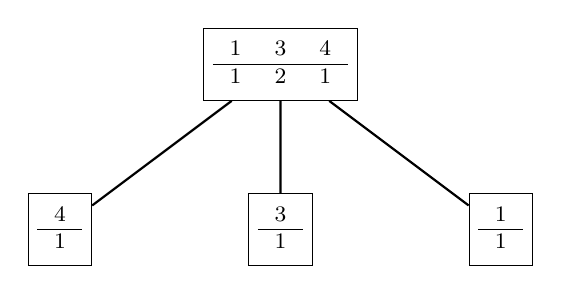
\begin{tikzpicture}[scale=0.7]

\node[draw, rectangle] (a) at (4,5.5)
{
\footnotesize
\begin{tabular}{rrr}
4 \\
\hline
1 \\
\end{tabular}};

\node[draw, rectangle] (b) at (8,5.5)
{
\footnotesize
\begin{tabular}{rrr}
3 \\
\hline
1 \\
\end{tabular}};


\node[draw, rectangle] (c) at (12,5.5)
{
\footnotesize
\begin{tabular}{rr}
1 \\
\hline
1 \\
\end{tabular}};

\node[draw, rectangle] (d) at (8,8.5)
{
\footnotesize
\begin{tabular}{rrr}
1 & 3 & 4 \\
\hline
1 & 2 & 1 \\
\end{tabular}};
\path[draw,thick,-] (a) -- (d);
\path[draw,thick,-] (b) -- (d);
\path[draw,thick,-] (c) -- (d);
\end{tikzpicture}
\end{center}

このようなデータ構造を各ノードに対して作成すれば、作成した直後にノードに関連するすべての問い合わせを処理することができ、与えられたすべての問い合わせを容易に処理することができます。
例えば 、ノード$4$に対する上記のマップ構造は、その部分木に値が3である2つのノ ードが含まれることがわかります。

ですが、これらすべてのデータ構造を一から作成するのは時間がかかりすぎます。
そこで、各ノード$s$において、$s$の値のみを含む初期データ構造$\texttt{d}[s]$を作成し、
その後に$s$の子を訪問して$u$が$s$の子であるすべてのデータ構造$\texttt{d}[u]$と$\texttt{d}[s]$をマージすることにします。
例えば、ノード$4$のマップは、以下のマップをマージして作成されています。

\begin{center}
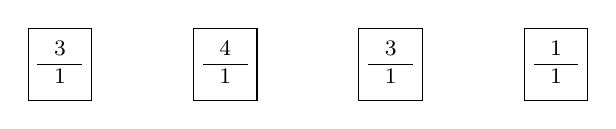
\begin{tikzpicture}[scale=0.7]

\node[draw, rectangle] (a) at (4,5.5)
{
\footnotesize
\begin{tabular}{rrr}
4 \\
\hline
1 \\
\end{tabular}};

\node[draw, rectangle] (b) at (7,5.5)
{
\footnotesize
\begin{tabular}{rrr}
3 \\
\hline
1 \\
\end{tabular}};

\node[draw, rectangle] (c) at (10,5.5)
{
\footnotesize
\begin{tabular}{rr}
1 \\
\hline
1 \\
\end{tabular}};

\node[draw, rectangle] (d) at (1,5.5)
{
\footnotesize
\begin{tabular}{rr}
3 \\
\hline
1 \\
\end{tabular}};

\end{tikzpicture}
\end{center}

ここでは、最初のマップがノード4の初期データ構造と、他の3つのマップ がそれぞれノード7、8、9に対応しています。

ノード$s$でのマージは次のようにします。
$s$の子を訪問し、各$u$で $\texttt{d}[s]$と$\texttt{d}[u]$をマージする。
$\texttt{d}[u]$から$\texttt{d}[s]$へは常に内容をコピーする。
この前に、$\texttt{d}[s]$が$\texttt{d}[u]$よりも小さければ、$\texttt{d}[s]$と$\texttt{d}[u]$の内容を入れ替える。
このようにすると、木の探索中に各値は$O(\log n)$回だけコピーされることになり、
この アルゴリズムは効率的に動作します。
2つのデータ構造a,bの内容を効率よく入れ替えるのは非常に簡単です。

\begin{lstlisting}
swap(a,b);
\end{lstlisting}
$a$ と $b$ が C++ 標準ライブラリのデータ構造であるとき、
上記のコードは定数時間で動作することが保証されています。

\subsubsection{LCA - Lowest common ancestors}

また、LCAのクエリを処理するオフラインのアルゴリズム\footnote{This
algorithm was published by R. E. Tarjan in 1979 \cite{tar79}.}もあります。
このアルゴリズムはunion-findデータ構造(第15.2章参照)に基づいており、
先ほどに説明したアルゴリズムよりも簡単に実装できます。

このアルゴリズムは、入力としてノードのペアのセットが与えられ両ノードのLCAを決定します。
まず、各ノードが別の集合に属する木を作り、深さ優先の木探索を行います。
初期状態では、各ノードは別々の集合に属している。
また、各集合に対して、その集合に属する木における最も高さが高い(根に近い)ノードを保存しておきます。

このアルゴリズムでは、$x$を訪問した時に、
$y$が既に訪問されているなら、
$y$の属する最も高いノードがLCAであると判断します。
そして、ノード$x$を処理した後、アルゴリズムは$x$とその親の集合を結合します。

(訳注: このアルゴリズムはオイラーツアーを行い、戻りの処理の際に親の集合との結合を行います。
そして、子側の集合の親は結合先の最も浅いノードだと情報を更新します。これはUnion-FindのLeaderに関して情報を持っておけば実装できます)

今、2つのクエリ $(5,8)$, $(2,7)$ を受けこのLCAを求めたいとします。
\begin{center}
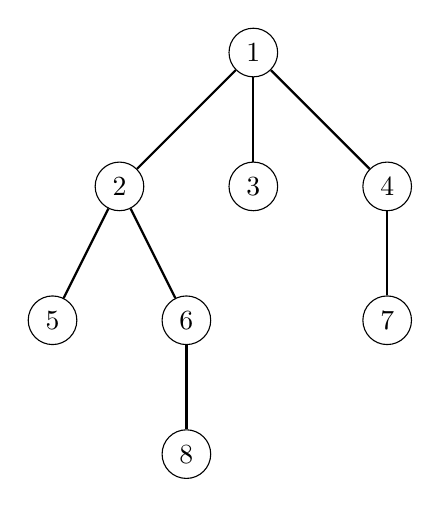
\begin{tikzpicture}[scale=0.85]
\node[draw, circle] (1) at (0,3) {$1$};
\node[draw, circle] (2) at (2,1) {$4$};
\node[draw, circle] (3) at (-2,1) {$2$};
\node[draw, circle] (4) at (0,1) {$3$};
\node[draw, circle] (5) at (2,-1) {$7$};
\node[draw, circle] (6) at (-3,-1) {$5$};
\node[draw, circle] (7) at (-1,-1) {$6$};
\node[draw, circle] (8) at (-1,-3) {$8$};
\path[draw,thick,-] (1) -- (2);
\path[draw,thick,-] (1) -- (3);
\path[draw,thick,-] (1) -- (4);
\path[draw,thick,-] (2) -- (5);
\path[draw,thick,-] (3) -- (6);
\path[draw,thick,-] (3) -- (7);
\path[draw,thick,-] (7) -- (8);
\end{tikzpicture}
\end{center}


次の図で灰色のノードは既に訪問したノードを表し、
破線で囲ったノードは同じ集合に属していることを示します。
アルゴリズムがノード8を訪問します。
この時にノード5が既に訪問済みであり、
その集合の中で最も高いノードは2であることに気づきます。
したがって、ノード5と8の最小公倍数の祖先は2となります。

\begin{center}
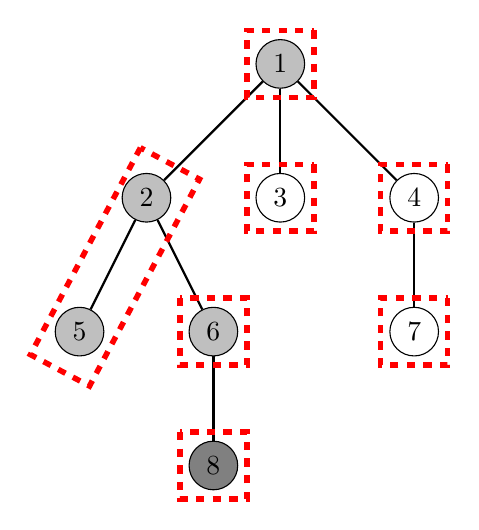
\begin{tikzpicture}[scale=0.85]
\node[draw, circle, fill=lightgray] (1) at (0,3) {$1$};
\node[draw, circle] (2) at (2,1) {$4$};
\node[draw, circle, fill=lightgray] (3) at (-2,1) {$2$};
\node[draw, circle] (4) at (0,1) {$3$};
\node[draw, circle] (5) at (2,-1) {$7$};
\node[draw, circle, fill=lightgray] (6) at (-3,-1) {$5$};
\node[draw, circle, fill=lightgray] (7) at (-1,-1) {$6$};
\node[draw, circle, fill=gray] (8) at (-1,-3) {$8$};
\path[draw,thick,-] (1) -- (2);
\path[draw,thick,-] (1) -- (3);
\path[draw,thick,-] (1) -- (4);
\path[draw,thick,-] (2) -- (5);
\path[draw,thick,-] (3) -- (6);
\path[draw,thick,-] (3) -- (7);
\path[draw,thick,-] (7) -- (8);

\draw [red,thick,dashed,line width=2pt,rotate around={-28:(-2,0)}] (-2.9,1.5) rectangle (-1.9,-2);


\draw [red,thick,dashed,line width=2pt] (-1.5,-0.5) rectangle (-0.5,-1.5);
\draw [red,thick,dashed,line width=2pt] (-1.5,-2.5) rectangle (-0.5,-3.5);

\draw [red,thick,dashed,line width=2pt] (0.5,3.5) rectangle (-0.5,2.5);
\draw [red,thick,dashed,line width=2pt] (0.5,1.5) rectangle (-0.5,0.5);
\draw [red,thick,dashed,line width=2pt] (2.5,1.5) rectangle (1.5,0.5);
\draw [red,thick,dashed,line width=2pt] (2.5,-0.5) rectangle (1.5,-1.5);
\end{tikzpicture}
\end{center}

探索を進めノード7に到着した時が次の木です。同様にLCAは1であることがわかりました。
\begin{center}
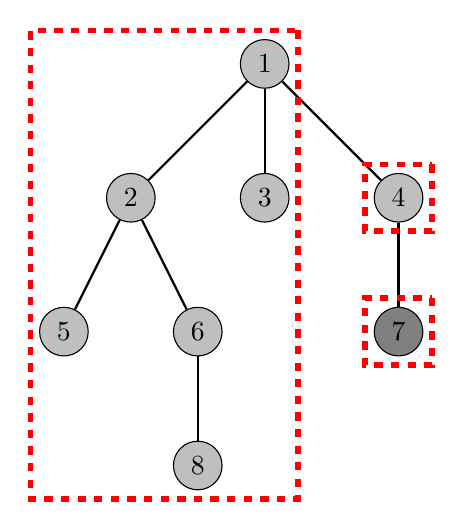
\begin{tikzpicture}[scale=0.85]
\node[draw, circle, fill=lightgray] (1) at (0,3) {$1$};
\node[draw, circle, fill=lightgray] (2) at (2,1) {$4$};
\node[draw, circle, fill=lightgray] (3) at (-2,1) {$2$};
\node[draw, circle, fill=lightgray] (4) at (0,1) {$3$};
\node[draw, circle, fill=gray] (5) at (2,-1) {$7$};
\node[draw, circle, fill=lightgray] (6) at (-3,-1) {$5$};
\node[draw, circle, fill=lightgray] (7) at (-1,-1) {$6$};
\node[draw, circle, fill=lightgray] (8) at (-1,-3) {$8$};
\path[draw,thick,-] (1) -- (2);
\path[draw,thick,-] (1) -- (3);
\path[draw,thick,-] (1) -- (4);
\path[draw,thick,-] (2) -- (5);
\path[draw,thick,-] (3) -- (6);
\path[draw,thick,-] (3) -- (7);
\path[draw,thick,-] (7) -- (8);

\draw [red,thick,dashed,line width=2pt] (0.5,3.5) rectangle (-3.5,-3.5);
\draw [red,thick,dashed,line width=2pt] (2.5,1.5) rectangle (1.5,0.5);
\draw [red,thick,dashed,line width=2pt] (2.5,-0.5) rectangle (1.5,-1.5);

\end{tikzpicture}
\end{center}
